\documentclass{article}


\usepackage{arxiv}

\usepackage[utf8]{inputenc} % allow utf-8 input
\usepackage[T1]{fontenc}    % use 8-bit T1 fonts
\usepackage{hyperref}       % hyperlinks
\usepackage{url}            % simple URL typesetting
\usepackage{booktabs}       % professional-quality tables
\usepackage{amsfonts}       % blackboard math symbols
\usepackage{nicefrac}       % compact symbols for 1/2, etc.
\usepackage{microtype}      % microtypography
\usepackage{lipsum}

\usepackage{graphicx}
\graphicspath{{../img/}}

\title{Using ML For Generating Cryptographic functions}


\author{
  David S.~Hippocampus\thanks{Use footnote for providing further
    information about author (webpage, alternative
    address)---\emph{not} for acknowledging funding agencies.} \\
  Department of Computer Science\\
  Cranberry-Lemon University\\
  Pittsburgh, PA 15213 \\
  \texttt{hippo@cs.cranberry-lemon.edu} \\
  %% examples of more authors
   \And
 Elias D.~Striatum \\
  Department of Electrical Engineering\\
  Mount-Sheikh University\\
  Santa Narimana, Levand \\
  \texttt{stariate@ee.mount-sheikh.edu} \\
  %% \AND
  %% Coauthor \\
  %% Affiliation \\
  %% Address \\
  %% \texttt{email} \\
  %% \And
  %% Coauthor \\
  %% Affiliation \\
  %% Address \\
  %% \texttt{email} \\
  %% \And
  %% Coauthor \\
  %% Affiliation \\
  %% Address \\
  %% \texttt{email} \\
}

\begin{document}
\maketitle

\begin{abstract}
TODO: read and review
In this paper we unite machine learning 
and cryptography: using ML methods 
trying to solve one of the 
most important problem
in cryptography: to find boolean
function with acceptable cryptological
properties. Neural network for making pseudorandom
function is developed. This function 
used as round function in Feistel Network, which 
 we finally test on NIST test battery.
\end{abstract}

\keywords{Cryptography \and Machine Learning \and Reinforcement Learning \and Privacy}



\section{Introduction}
TODO: read and review
Cryptography is widely used in
information security. 
Everyone is using it in messagers, shops, 
in internet of things and many others 
aspects of life. Many users
encrypt its personal data without even 
knowing what cryptography is. 

There are a lot of basic templates
for cryptographic encryption
functions called schemes - Feisteil network, SP-network, XSL-scheme etc. 
Every scheme has adjustable
set of parameters such as 
plaintext and key size, internal
round functions, number of rounds. 
Best practice in constructing new encryption
algorithm is to choose a good scheme, 
then select perfect parameters of chosen scheme.
For example, algorithm AES is a XSL-scheme 
with choosen internal operations, including s-boxes.

Chosing excellent round functions in another part 
of cryptographic art.
When new algorithm is published,
researchers of whole world trying to find 
 weakness in it.
 Besides, absence of attacks 
 doesn't mean that algorithm is strong. 
 Many people, besides,  prefer  concept of 
 <<nothing up my sleeve numbers>> \cite{NMSN}, 
 which require generating s-boxes only 
 by random choise. Otherwise one can say that you
 try to hide specific propeties of your algorithm.
 
 
 On the other hand, ML methods can be applying as
 approach to find a good 
 
 That's why in this paper we use neuronal network for generating good round function 
 for Feisteil Network - one of the most popular scheme.
 Then we test properties of our algorithm on the NIST test battery.



\section{Symmetric encryption basics}
TODO...



\section{Problem statement}
TODO: read and review
From ancient times to nowadays 
many different types of 
cryptographic attacks were presented.
That's why cypher's developers very carefully 
selected cypher's parameters. 
Widely distributed (but, obviously, 
not absolutily reliable)
method of proving new cipher's security is 
trying to apply to it all 
known attacks. Impossibility
of applying all these attacks 
with acceptable time and data complexity
gives grounds to consider the cipher as
stable one. 

This method has a lot of 
obvious defects. 
On the one hand, many variety 
of new attacks developed 
every year (and not all of them 
are published). On the other hand, 
when developer examined cipher made
himself, he could miss some 
cipher's vulnerability. So 
you cannot say about 
absolute security.

Another look for cipher's security
if to make its encryption function 
indistinguishable from 
random substitution. 



\section{Reinforcement Learning}
TODO...



\section{Solution}
\subsection{Main idea}
TODO: (general words about combining encryption and ML)...

\subsection{Feisteil Network}
TODO: read and review
For our experiments we chose the 
Feisteil Network scheme. This scheme 
first published in []. It uses in previous 
international standard DES [] and present
widely used algorithm GOST28147-89 []. 
Now we'll give a brief discription of the scheme.

Denote 
$X = (x_n, x_{n-1}, \dots, x_0), x_i \in \{0,1\}, i = 0, 1, \dots, n-1$ as
 input text, and 
$n$ as (so, also a cipher text) size.

One {\it round} of the scheme is to 
modify input text  $X = (X_l, X_r)$ 
to $$(X_r, X_l \oplus f(X_r, k)).$$

Scheme has fixed number of rounds, which 
we denote as $R$. 
Input of first round is the input text.
For other rounds input is the output of 
previous round. Cipher text is the output 
of the last ($R$-th) round.


then modify right part $X_r$ with 
function $f:V_{n/2}\rightarrow V_{n/2}$ and 
round key $k\in V_{n/2}$.

TODO: in our experiments we used the following settings:
Block size - 64 bit (2 x 32)
Rounds number - 16

\subsection{Neural network architecture}
TODO...
Deep fully connected network (8 layers), activation function - SELU
Stochastic computation graph

\subsection{Optimization approach}
TODO (Stochastic Policy Gradients, REINFORCE???)...

\subsection{Reward function}
TODO...
consists of 3 components, each corresponding to a class of well-known attacks on cryptographic functions:
Attack on related open texts
Attack on related keys
Attack on related encrypted texts

\subsection{Putting pieces together}
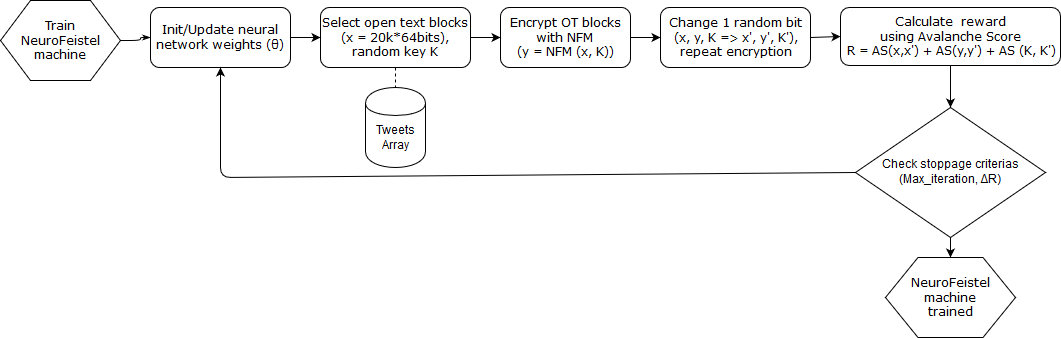
\includegraphics[scale=1]{img/NFM_learing.png}



\section{Experiments}
\subsection{Test methodology}
TODO...
Input text data - 10 million Twitter messages
Randomly generated round keys

\subsection{Validation}
TODO...
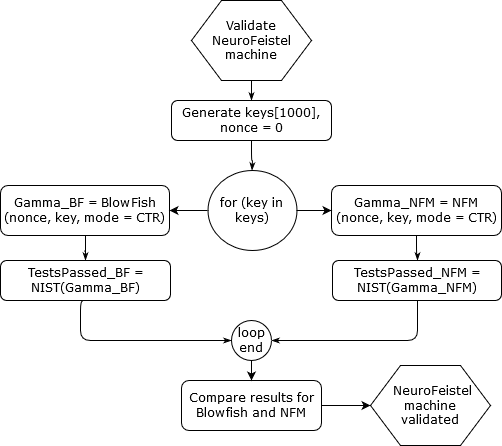
\includegraphics[scale=1]{img/NFM_validation.png}

\subsection{Results}
TODO...
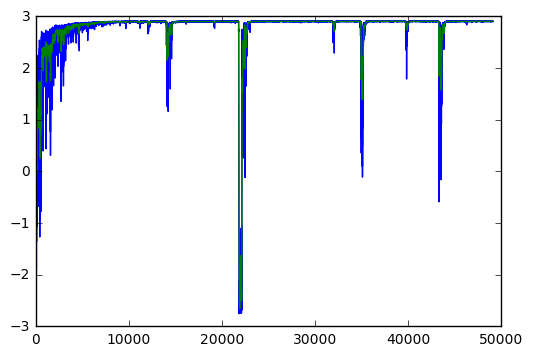
\includegraphics[scale=1]{img/learning_curve.png}
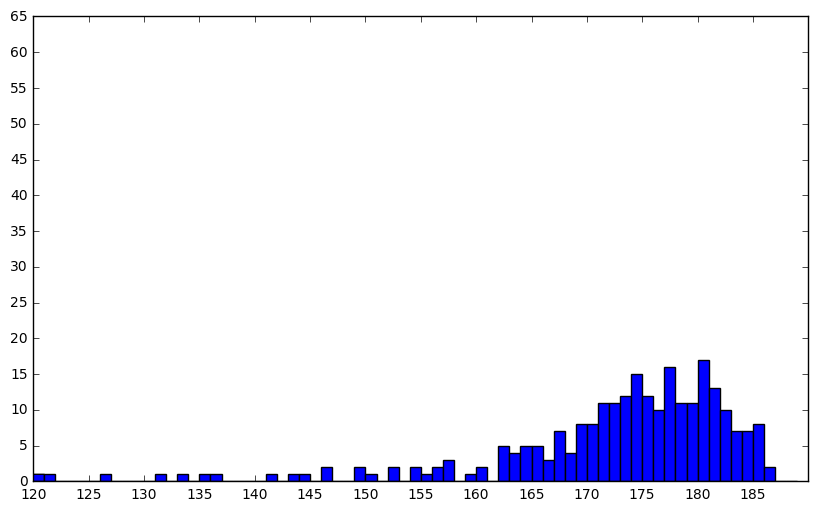
\includegraphics[scale=1]{img/result_nfm.png}
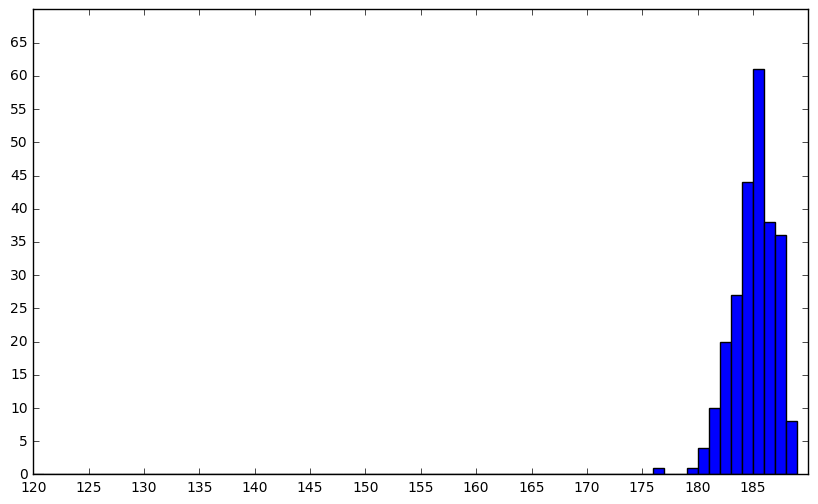
\includegraphics[scale=1]{img/result_blowfish.png}



\section{Thoughts on further development}
TODO...



\section{Conclusion}
TODO...



\bibliographystyle{unsrt}
\bibliography{references}

\end{document}
